\chapter{Исследовательская часть}

В данном разделе будут приведены примеры работы программы, а также проведен сравнительный анализ алгоритмов при различных ситуациях на основе полученных данных.

\section{Технические характеристики}

Технические характеристики устройства, на котором выполнялся эксперимент представлены далее:

\begin{enumerate}[label=\arabic*)]
	\item операционная система --- Ubuntu 22.04.3~\cite{ubuntu} Linux x86\_64;
	\item память --- 16 Гб;
	\item процессор --- Intel® Core™ i5-1135G7 @ 2.40 ГГц.
\end{enumerate}

При эксперименте ноутбук не был включен в сеть электропитания.

\section{Демонстрация работы программы}

На рисунке \ref{fig:example_linear} представлен результат работы программы при линейной обработке, а на рисунке \ref{fig:example_con} -- при конвейерной.

\begin{figure}[h!]
	\centering
	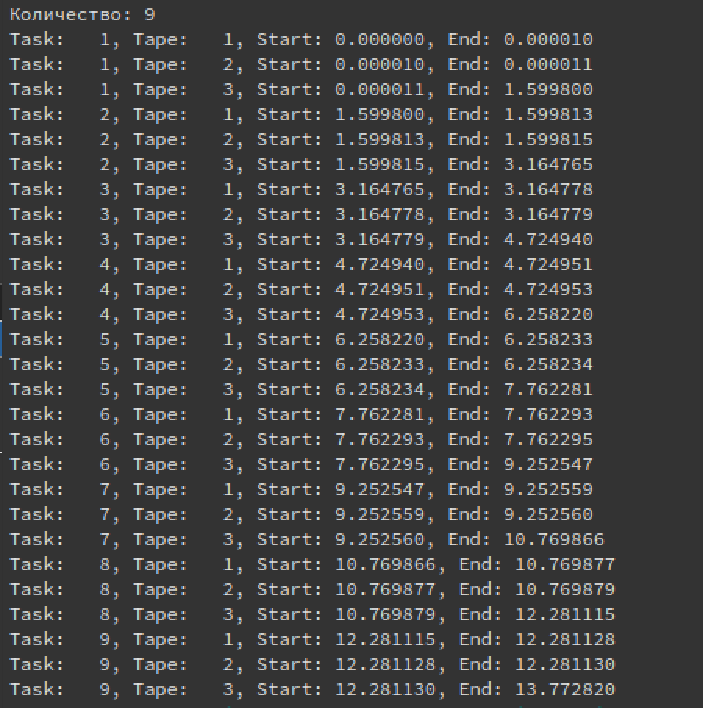
\includegraphics[width=0.6\linewidth]{img/example_linear}
	\caption{Пример работы программы (линейная)}
	\label{fig:example_linear}
\end{figure}

\begin{figure}[h!]
	\centering
	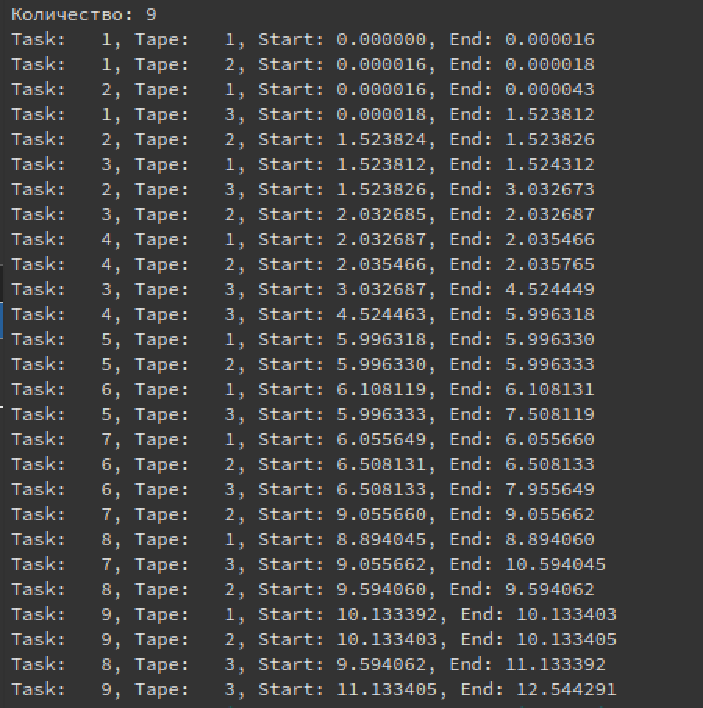
\includegraphics[width=0.6\linewidth]{img/example_con}
	\caption{Пример работы программы (конвейерная)}
	\label{fig:example_con}
\end{figure}
\clearpage

\section{Время выполнения алгоритмов}

Как было сказано выше, используется функция замера процессорного времени \textit{std::chrono::system\_clock::now(...)} из библиотеки $chrono$ на C++. 
Функция возвращает процессорное время типа float в секундах.

Функция используется дважды: перед началом выполнения алгоритма и после завершения, затем из конечного времени вычитается начальное, чтобы получить результат.

Замеры проводились для разного размера файлов, а также для разного количества файлов, чтобы определить, когда наиболее эффективно использовать конвейерную обработку.

Результаты замеров приведены в таблицах \ref{tbl:time_lin_count}-\ref{tbl:time_conv_size} (время в мс).

\begin{table}[h]
    \begin{center}
        \begin{threeparttable}
        \captionsetup{justification=raggedright,singlelinecheck=off}
        \caption{Результаты замеров времени (линейная, разное количество файлов)}
        \label{tbl:time_lin_count}
        \begin{tabular}{|p{6cm}|p{6cm}|}
            \hline
            Кол-во матриц & Время \\
            \hline
            1 & 1.5238 \\ \hline 
            2 & 3.0126 \\ \hline 
            3 & 4.4944 \\ \hline 
            4 & 5.9263 \\ \hline 
            5 & 7.4181 \\ \hline 
            6 & 8.9156 \\ \hline 
            7 & 10.2940 \\ \hline 
            8 & 11.9333 \\ \hline 
            9 & 13.2111 \\ \hline  
		\end{tabular}
    \end{threeparttable}
\end{center}
\end{table}


\begin{table}[h]
    \begin{center}
        \begin{threeparttable}
        \captionsetup{justification=raggedright,singlelinecheck=off}
        \caption{Результаты замеров времени (конвейeрная, разное количество файлов)}
        \label{tbl:time_conv_count}
        \begin{tabular}{|p{6cm}|p{6cm}|}
            \hline
            Кол-во матриц & Время \\
            \hline
            1 & 1.1238 \\ \hline 
            2 & 2.2126 \\ \hline 
            3 & 3.4932 \\ \hline 
            4 & 4.9264 \\ \hline 
            5 & 6.1183 \\ \hline 
            6 & 7.2151 \\ \hline 
            7 & 8.4947 \\ \hline 
            8 & 9.4323 \\ \hline 
            9 & 10.1131 \\ \hline
		\end{tabular}
    \end{threeparttable}
\end{center}
\end{table}


\begin{table}[h]
    \begin{center}
        \begin{threeparttable}
        \captionsetup{justification=raggedright,singlelinecheck=off}
        \caption{Результаты замеров времени (линейная, разные размеры файлов)}
        \label{tbl:time_lin_size}
        \begin{tabular}{|p{6cm}|p{6cm}|}
            \hline
            Размер матриц & Время \\
            \hline
            100 & 1.5238 \\ \hline 
            200 & 2.2589 \\ \hline 
            300 & 3.3409 \\ \hline 
            400 & 4.3925 \\ \hline 
            500 & 5.5193 \\ \hline 
            600 & 6.7832 \\ \hline 
            700 & 7.6820 \\ \hline 
            800 & 8.9341 \\ \hline 
            900 & 9.2402 \\ \hline 
		\end{tabular}
    \end{threeparttable}
\end{center}
\end{table}


\begin{table}[h]
    \begin{center}
        \begin{threeparttable}
        \captionsetup{justification=raggedright,singlelinecheck=off}
        \caption{Результаты замеров времени (конвейерная, разные размеры файлов)}
        \label{tbl:time_conv_size}
        \begin{tabular}{|p{6cm}|p{6cm}|}
            \hline
            Размер & Время \\
            \hline 
            100 & 1.1238 \\ \hline 
            200 & 1.5573 \\ \hline 
            300 & 1.9623 \\ \hline 
            400 & 2.8435 \\ \hline 
            500 & 3.6133 \\ \hline 
            600 & 4.6842 \\ \hline 
            700 & 5.3834 \\ \hline 
            800 & 6.4346 \\ \hline 
            900 & 7.1013 \\ \hline 
		\end{tabular}
    \end{threeparttable}
\end{center}
\end{table}

\clearpage

Также на рисунках \ref{fig:graph_count}--\ref{fig:graph_size} приведены графические результаты замеров.

\begin{figure}[h!]
	\centering
	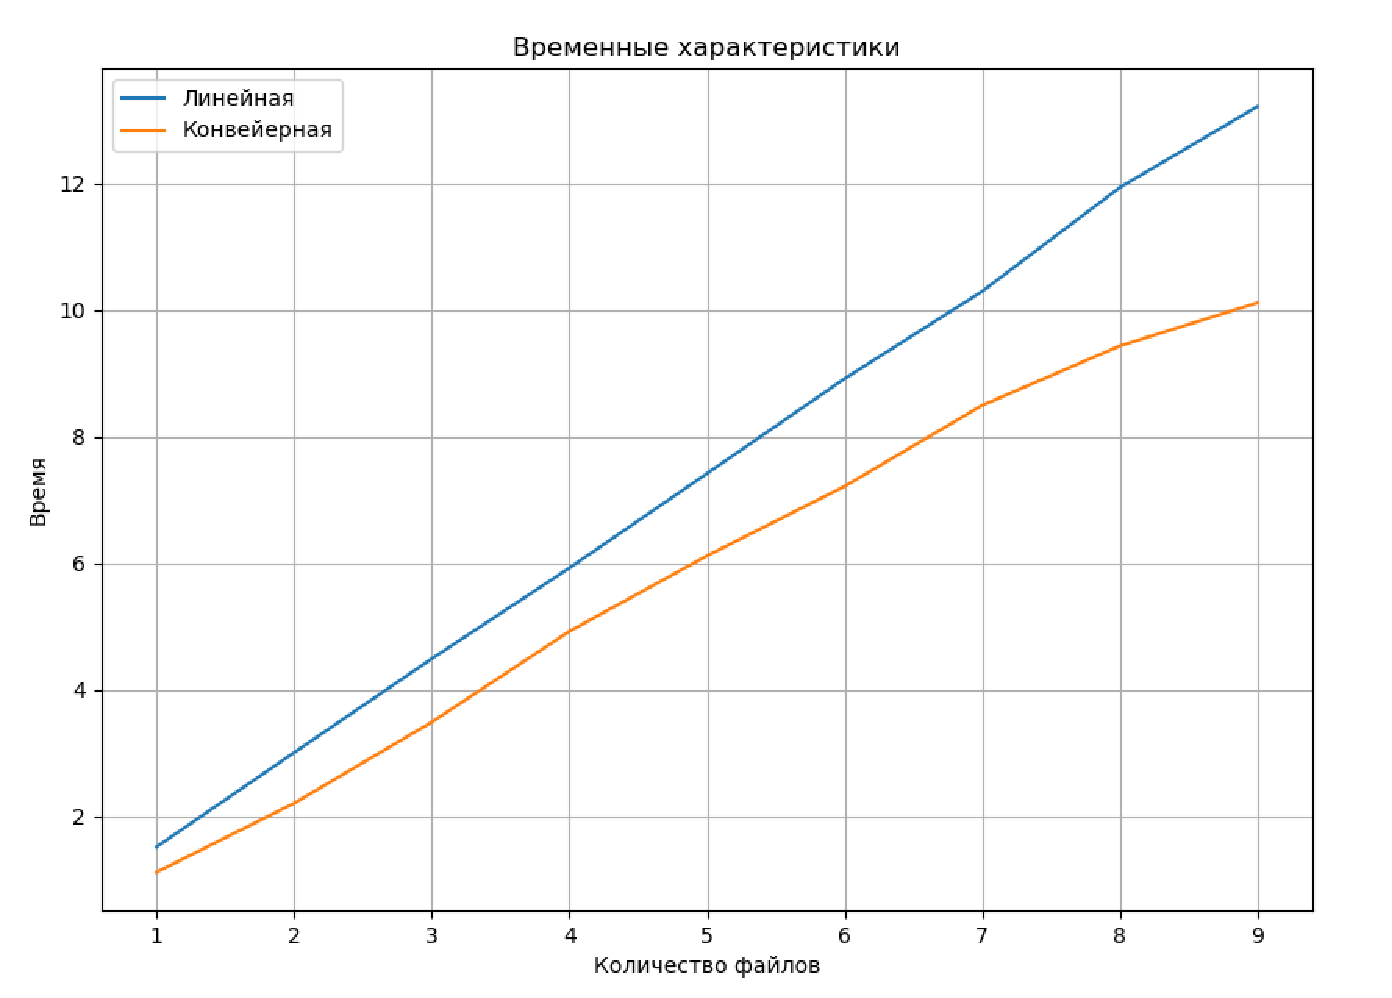
\includegraphics[width=0.8\linewidth]{img/graph_count}
	\caption{Сравнение по времени линейной и конвейерной обработок для разного количества файлов}
	\label{fig:graph_count}
\end{figure}

\begin{figure}[h!]
	\centering
	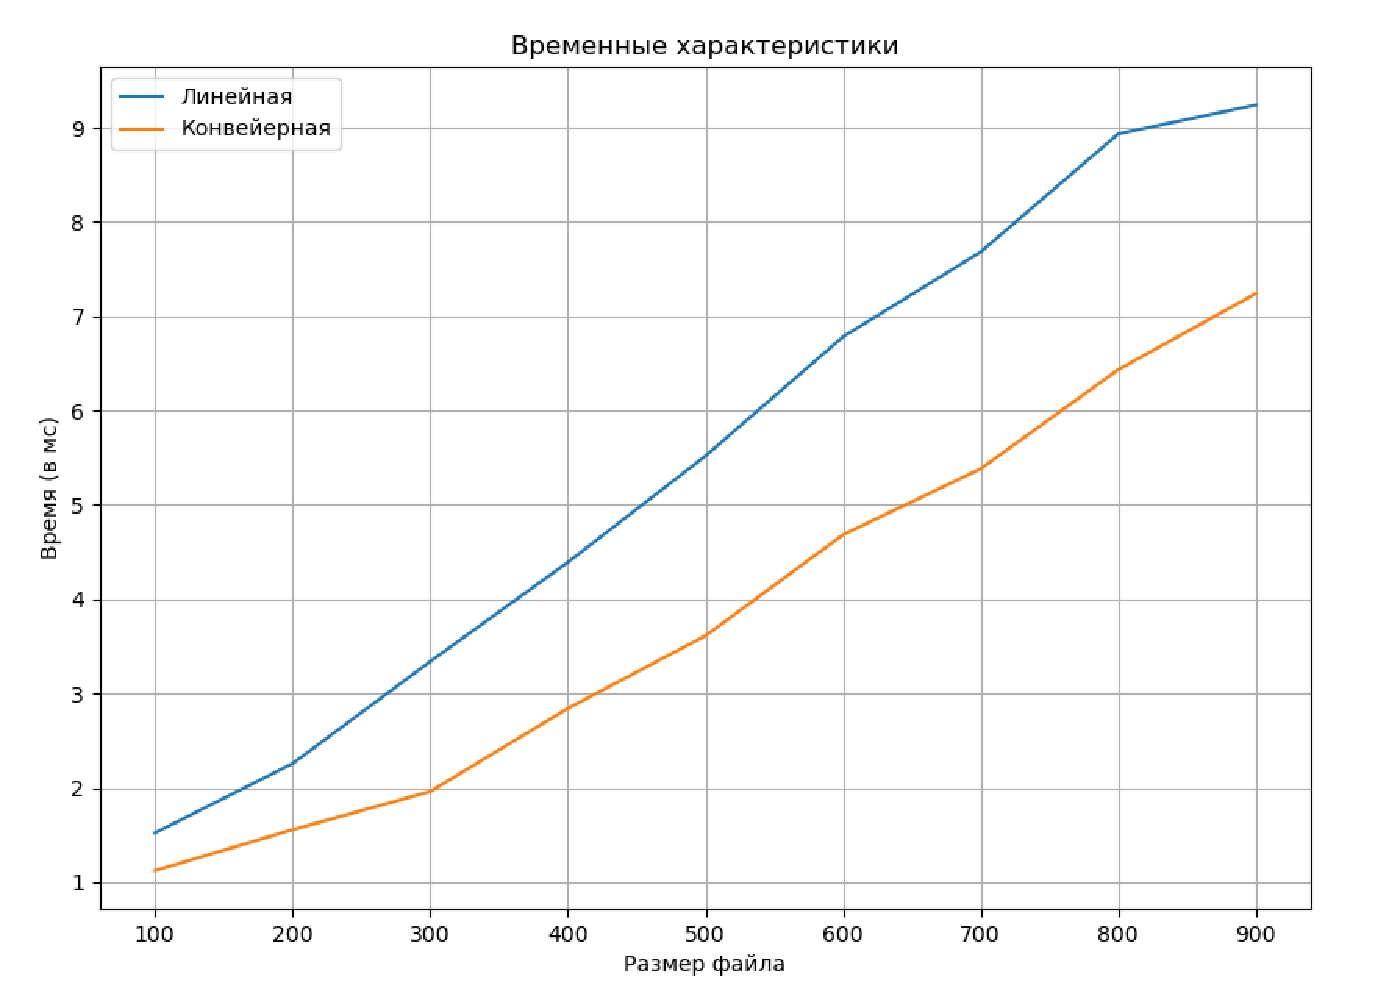
\includegraphics[width=0.8\linewidth]{img/graph_size}
	\caption{Сравнение по времени линейной и конвейерной обработок для разных размеров файлов}
	\label{fig:graph_size}
\end{figure}

\clearpage


\section{Вывод}

В результате эксперимента было получено, что при использовании конвейерной обработки время выполенения меньше, чем при линейной реализации при количестве файлов, равном 4, в 1.2 раза, а при количестве файлов, равном 9, уже в 1.3 раза. 
Следовательно, конвейерная реализация лучше линейной при увеличении количества задач (файлов).

Также при проведении эксперимента было выявлено, что при увеличении размера файла конвейерная реализация выдает лучшие результаты. 
Так, при размере файла в 100 кб конвейерная реализация быстрее в 1.2 раза, чем линейная, а при размере файла, равном 900 кб, в 1.3 раза. 